\documentclass[11pt]{article}
\usepackage[scaled=0.92]{helvet}
\usepackage{geometry}
\geometry{letterpaper,tmargin=1in,bmargin=1in,lmargin=1in,rmargin=1in}
\usepackage[parfill]{parskip} % Activate to begin paragraphs with an empty line rather than an indent %\usepackage{graphicx}
\usepackage{amsmath,amssymb, mathrsfs, dsfont}
\usepackage{tabularx}
\usepackage[all,cmtip]{xy}
\usepackage[font=footnotesize,labelfont=bf]{caption}
\usepackage{graphicx}
\usepackage{xcolor}
%\usepackage[linkbordercolor ={1 1 1} ]{hyperref}
%\usepackage[sf]{titlesec}
\usepackage{natbib}
%\usepackage{tikz-cd}

\usepackage{../../Tianpei_Report}

%\usepackage{appendix}
%\usepackage{algorithm}
%\usepackage{algorithmic}

%\renewcommand{\algorithmicrequire}{\textbf{Input:}}
%\renewcommand{\algorithmicensure}{\textbf{Output:}}



\begin{document}
\title{Lecture 2: Probably Approximately Correct Learning}
\author{ Tianpei Xie}
\date{ Jul. 30th., 2015 }
\maketitle
\tableofcontents
\newpage
\section{PAC Learning for Realizable Case}
\subsection{Definitions}
\begin{itemize}
\item \begin{remark} (\emph{Settings}) \\
\emph{In deterministic scenario}, denote a collection of $n$ \emph{independent identically distributed (i.i.d.) \textbf{random samples}} generated by $P_X$ as $X = \paren{X_1 \xdotx{,} X_n}$, and \emph{label} is generated from a concept $c \in \cC$ as $Y_i = c(X_i)$. Denote the sample as 
\begin{align*}
\cD \equiv \cD_n = \paren{(X_1, Y_1) \xdotx{,} (X_n, Y_n)} \equiv  \paren{(X_1, c(X_1)) \xdotx{,} (X_n, c(X_n))} .
\end{align*} Thus, $\cD_n|_{X} \sim \cP_X^n$ is a random sequence of $n$ i.i.d. samples.

A \underline{\emph{\textbf{learner}}} $\cA$  considers a \emph{\textbf{fixed} subset of concepts}  $\cH\subset \cC$, which is referred as a \underline{\emph{\textbf{hypothesis class}}}, and provides a \emph{\textbf{hypothesis}} or a \underline{\emph{\textbf{classifier}}} or a \emph{\textbf{decision function}} $h\in \cH$. The task of \underline{\emph{\textbf{supervised learning}}} is to minimize \emph{the generalization error}:
\begin{align*}
L(h) \equiv L_{\cP, c}(h) &= \cP_{X}\set{h(X) \neq c(X)} \equiv \E{\cP}{\mathds{1}_{h(X)\neq c(X)}}
\end{align*} where $\mathds{1}_{\omega}$ is the indicator function of the event $\omega$. 

In particular, \emph{a learning algorithm (such as ERM)} $\cA$ takes sample $\cD_n$ as input and output 
\begin{align*}
\cA(\cD_n) = h_n =  h_{\cD_n}^{*}(x)  \equiv  h(x | ((X_1, Y_1) \xdotx{,} (X_n, Y_n)) ).
\end{align*}  Given that $\cD_n$ are random samples, \emph{\textbf{$h_n \equiv h_{\cD_n}$ are random}} as well. Thus \emph{\textbf{the generalization error}} of $h_n$ is a \emph{\textbf{random variable}}: 
\begin{align*}
L_n \equiv L_{\cP, c}(h_n) := \E{}{ \ind{h_{\cD_n}(X) \neq c(X)}| \cD_n} = \cP\set{h_{\cD_n}(X) \neq c(X) | \cD_n}.
\end{align*}
\end{remark}


\item  \begin{remark}
We denote by $\cO(d)$ an \emph{upper bound} on \emph{the \textbf{cost} of the \textbf{computational representation}} of any element $x \in \cX \subset \bR^d$ and by $\text{size}(c)$ \emph{\textbf{the maximal cost} of the computational representation of $c \in \cC$}. For example, $x$ may be a vector in $\bR^d$,
for which the cost of an array-based representation would be in $\cO(n)$.
\end{remark}

\item \begin{remark}(\textbf{\emph{Realizability Assumption}})\\
There exists a hypothesis $h \in \cH$ such that \emph{\textbf{the generalization error is zero}}.
\begin{align*}
\exists h\in \cH, \quad  L_{\cP, c}(h) = 0
\end{align*} \emph{\textbf{Every ERM hypothesis has zero training error}}. In the definition of \emph{\textbf{Probably Approximately Correct (PAC) Learning}}, we assume the realizability assumption holds.
\end{remark}

\item 
\begin{definition} (\emph{\textbf{Probably Approximately Correct (PAC) Learning, Realizable Case}})\\
Assume that \emph{the realizability assumption holds}. A \emph{hypothesis class} $\cH$  is said to be \underline{\emph{\textbf{Probably}}} \underline{\emph{\textbf{Approximately Correct-learnable}}} i.e. \underline{\emph{\textbf{PAC-learable}}},  if there exists an \emph{algorithm} $\cA$ and a \emph{\textbf{polynomial function}} $\text{poly}(\cdot, \cdot, \cdot, \cdot)$  such that for any $\epsilon > 0$ and $\delta > 0$, for \emph{\textbf{all distributions}} $\cP$ on $\cX$ and \emph{for any target concept} $c \in \cC$, %and if \emph{\textbf{the realizable assumption holds}} with respect to $\cH$, $\cP$, $c$, then 
 the following holds when the \emph{\textbf{sample size}} $n \ge \text{poly}(1/\epsilon, 1/\delta, d, \text{size}(c)):$
\begin{align}
\cP\set{L_{\cP, c}(\cA(\cD_n))  \le \epsilon} &\ge  1 - \delta.  \label{eqn: pac_definition}
\end{align}
If $\cA$ further runs in $\text{poly}(1/\epsilon, 1/\delta, d, \text{size}(c))$, then $\cH$ is said to be \underline{\emph{\textbf{efficiently PAC-learnable}}}. When such an algorithm $\cA$ exists, it is called a \emph{\textbf{PAC-learning algorithm}} for $\cH$.
\end{definition}

%\item \begin{remark} 
%We can use the  for any $\epsilon, \delta >0$, any distributions $\cP$ and any concept $c\in \cC$, denote the decision function returned by the learning algorithm after receiving $n$ samples from $\cP$ as $h_n$, then when $n \ge  \text{poly}(1/\epsilon, 1/\delta, d, \text{size}(c))$, \emph{\textbf{with probability at least}} $1 - \delta$
%\begin{align*}
%L_{\cP, c}(h_n) \le \epsilon.
%\end{align*}
%\end{remark}

\item \begin{remark}
\emph{A hypothesis class} $\cH$ is thus \emph{\textbf{PAC-learnable}} if the hypothesis returned by the algorithm after observing a number of points \emph{\textbf{polynomial}} in $1/\epsilon$ and $1/\delta$ is
\begin{enumerate}
\item \emph{\textbf{approximately correct}} (\emph{error at most $\epsilon$}) 
\item \emph{\textbf{with high probability}} (at least $1 - \delta$), 
\end{enumerate}
which justifies \emph{the PAC terminology}. 
\begin{enumerate}
\item $\delta > 0$ is used to define \emph{\textbf{the confidence}} $1 - \delta$
\item and $\epsilon > 0$ \emph{\textbf{the accuracy}} $1-\epsilon$. 
\end{enumerate}
Note that if the running time of the algorithm is \emph{\textbf{polynomial}} in $1/\epsilon$ and $1/\delta$, then \emph{\textbf{the sample size}} $n$ must also be polynomial if the full sample is received by the algorithm.
\end{remark}

\item \begin{remark} (\textbf{\emph{Confidence} and \emph{Accuracy}})
\begin{enumerate}
\item For a fixed classifer $h$, \emph{the \textbf{accuracy} of that classifer} is measured by $1 - L_{\cP, c}(h)$. 

\item The \emph{\textbf{confidence}} of \emph{\textbf{learning algorithm}} is measured by \emph{\textbf{the probability of failure} for hypothesis returned by the learning algorithm}. A failure happens when the learned classifier $h$ has \emph{\textbf{low accuracy}}, i.e. $L_{\cP, c}(h) > \epsilon$. Since classifer $h_{\cD}$ is function of data $\cD_n$, the \emph{confidence} is measured by \emph{\textbf{the probability of encountering bad samples}} $\cD_n$ such that $\widehat{L}_{\cD}(h_{\cD}) = 0$ but $L_{\cP, c}(h_{\cD}) > \epsilon$.
\end{enumerate}
$\cH$ is \emph{\textbf{PAC-learnable}} when a learning algorithm has \emph{\textbf{high confidence}} to obtain a classifier $h \in \cH$ with \emph{\textbf{high accuracy}} \emph{\textbf{regardless}} of the underlying \emph{\textbf{data distribution}} and \emph{\textbf{labeling logic}}.
\end{remark}


\item \begin{remark}
Several key points of the PAC definition are worth emphasizing. 
\begin{enumerate}
\item First, \emph{the PAC framework is a \underline{\textbf{distribution-free}}}: \emph{no particular assumption} is made about \emph{the distribution $\cP$} from which examples are drawn. 

\item Second, \emph{the training sample} and \emph{the test examples} used to define the error are drawn \emph{according to \textbf{the same distribution} $\cP$}. This is a necessary assumption for generalization to be possible in most cases.

\item Third, the PAC framework is \underline{\emph{\textbf{non-asymptotic}}} in which it provides \emph{a \textbf{concentration inequality}} that holds for all $n$. %The \emph{asymptotic results} such as \emph{\textbf{universal consistency}} holds true if the PAC learnability is true.

\item Finally, \emph{the PAC framework deals with the question of \textbf{learnability for a hypothesis class} $\cH$ and not a particular hypothesis $h$}. Note that \emph{\textbf{the concept class $\cC$ is known to the algorithm}}, but of course target concept $c \in \cC$ is unknown.
\end{enumerate}
We may omit the polynomial dependency on $n$ and $\text{size}(c)$ in the PAC definition and \emph{focus only on the \textbf{sample complexity}}.
\end{remark}
\end{itemize}

\subsection{PAC-Learnable Guarantees for Finite Hypothesis Sets}
\begin{itemize}
\item \begin{remark} (\emph{\textbf{Finite Hypothesis Sets}})\\
We will see if the size of hypothesis class $\cH$ is finite, i.e. $\abs{\cH} < \infty$, we can achieve \emph{PAC learnability} under \emph{the realizability assumption}:
\end{remark}

\item \begin{proposition} (\textbf{Learning bounds, Finite $\cH$, Realizable Case}) \citep{mohri2018foundations}\\
Let $\cH$ be a \textbf{finite} set of functions mapping from $\cX$ to $\cY$. Let $\cA$ be an algorithm that for \textbf{any target concept $c \in \cH$} and i.i.d. sample $\cD_n$ returns a consistent hypothesis $h_n$, i.e. \textbf{the training error of $h_n$ is zero}: $\widehat{L}(h_n) = 0$.
Then, for any $\epsilon, \delta > 0$, the inequality 
\begin{align*}
\cP^{n}\set{ L_{\cP, c}(h_n) \le \epsilon} &\ge  1 - \delta
\end{align*} holds if
\begin{align}
n &\ge \frac{1}{\epsilon}\log\paren{\frac{\abs{\cH}}{\delta}} \label{eqn: pac_sample_complexity_finite_case}
\end{align}
This sample complexity result admits the following \textbf{equivalent statement} as a generalization bound: for any $\epsilon, \delta > 0$, with \textbf{probability} at least $1 - \delta$,
\begin{align}
L_n \equiv L_{\cP, c}(h_n) &\le \frac{1}{n}\log\paren{\frac{\abs{\cH}}{\delta}}. \label{eqn: pac_sample_complexity_finite_case_consistency}
\end{align}
\end{proposition}
\begin{proof}
We want to upper bound the probability of event 
\begin{align*}
M := \set{\cD_n \sim \cP^n: \exists h \in \cH, \;\; L_{\cP, c}(h) > \epsilon \land \widehat{L}(h) = 0}.
\end{align*} In other word, for each sample $\cD_n \in M$, there are bad hypothesis that seems good in the training data $\cD_n$. Under the realizablity assumption, all samples that makes $ L_{\cP, c}(h_n) > \epsilon$ lies in $M$. Moreover, $M$ can be rewritten as
\begin{align*}
M = \bigcup_{h \in \cH_B}\set{\cD_n \sim \cP^n:  \widehat{L}(h) = 0}
\end{align*} where $\cH_B := \set{h \in \cH: \;\; L_{\cP, c}(h) > \epsilon}$. Then by union bound,
\begin{align}
\cP^n\set{L_{\cP, c}(h_{\cD_n }) > \epsilon} &\le  \cP^n\set{ \bigcup_{h \in \cH_B}\set{\cD_n:  \widehat{L}(h) = 0}}  \nonumber\\
&\le \sum_{h \in \cH_B}\cP^n\set{\cD_n:  \widehat{L}(h) = 0} \label{ineqn: finite_pac_union_bound}
\end{align} Note that 
\begin{align*}
\cP^n\set{\cD_n:  \widehat{L}(h) = 0} &= \cP^n\set{h(X_i) = c(X_i), i =1 \xdotx{,} n}\\
&= \prod_{i=1}^{n}\cP\set{h(X_i) = c(X_i)}
\end{align*} For each individual sampling of an element of the training set we have
\begin{align*}
\cP\set{h(X_i) = c(X_i)} &= 1 - L_{\cP, c}(h) \le 1- \epsilon
\end{align*} where the last inequality follows from the fact that $h \in \cH_B$. Thus, for all $h \in \cH_B$,
\begin{align*}
\cP^n\set{\cD_n:  \widehat{L}(h) = 0} &\le (1 - \epsilon)^n \le \exp\paren{- n \epsilon}
\end{align*} where the last inequality comes from $1 - x \le e^{-x}$. Combining this equation with \eqref{ineqn: finite_pac_union_bound} we conclude that
\begin{align*}
\cP^n\set{L_{\cP, c}(h_{\cD_n }) > \epsilon} &\le  \abs{\cH_B}\exp\paren{- n \epsilon} \le \abs{\cH}\exp\paren{- n \epsilon}.
\end{align*} Setting the right-hand side to be equal to $\delta$ and solving for $\epsilon$ concludes the proof. \qed
\end{proof}

\begin{figure}
\begin{minipage}[t]{1\linewidth}
  \centering
  \centerline{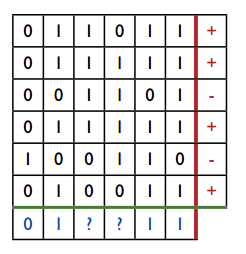
\includegraphics[scale = 0.6]{conjunction_boolean_literals.png}}
\end{minipage}
\caption{\footnotesize{\textbf{Algorithm to find concept behind the conjunction of boolean literals under realizability assumption \citep{mohri2018foundations}}}}
\label{fig: conjunction_boolean_literals}
\end{figure}


\item \begin{example}(\emph{\textbf{Conjunction of Boolean Literals}}) \citep{mohri2018foundations}\\
Consider learning the concept class $\cC_n$ of \underline{\emph{\textbf{conjunctions of at most $n$ Boolean literals}}} $x_1 \xdotx{,} x_n$. \underline{\emph{\textbf{A Boolean literal}}} is either a variable $x_i, i \in [1, n]$, or its \emph{negation} $\neg x_i$. For $n = 4$, an example is the conjunction: $x_1 \land \neg x_2 \land x_4$, where $\neg x_2$ denotes the negation of the Boolean literal $x_2$.  $(1, 0, 0, 1)$ is a \emph{positive example} for this concept ($1 \land \neg 0 \land 1 = 1$) while $(1, 0, 0, 0)$ is a \emph{negative} example ($1 \land \neg 0 \land 0 = 0 $).

\begin{remark}[\textit{\textbf{Algorithm}}] For each \emph{\textbf{positive example}} $(b_1 \xdotx{,} b_n)$and $i \in [1, n]$, if $b_i = 1$ then $\neg x_i$ is \emph{\textbf{ruled out}} as a possible literal in the concept class and if $b_i = 0$ then $x_i$ is ruled out. The conjunction of all the literals \emph{\textbf{not ruled out}} is thus \emph{a hypothesis \textbf{consistent with the target}}. 
\end{remark}

Figure \ref{fig: conjunction_boolean_literals} shows an example when $n = 6$. Each of the first six rows of the table represents a \emph{training example} with
its label, $+$ or $-$, indicated in the last column. The last row contains $0$ (respectively $1$) in column $i \in [1, 6]$ if the $i$-th entry is $0$ (respectively $1$) for all the positive examples. It contains ``?" if both $0$ and $1$ appear as an $i$-th entry for some positive example. Thus, for this training sample, the hypothesis returned by the consistent algorithm described in the text is $\neg x_1 \land x_2 \land x_5 \land x_6$.

We have $\abs{\cH} = \abs{\cC_n} = 3^n$, since each literal can be included \emph{positively}, \emph{with negation}, or \emph{not included}. Using the result of PAC Learning with realizability assumption, we see that for any $\epsilon > 0, \delta >0$, 
\begin{align*}
n \ge  \frac{1}{\epsilon}\log\paren{\frac{\abs{\cH}}{\delta}} =  \frac{1}{\epsilon}\paren{n\log3 - \log\delta} 
\end{align*} Thus, \emph{\textbf{the class of conjunctions of at most $n$ Boolean literals}} is \emph{\textbf{PAC-learnable}}. Note that the computational complexity is also polynomial, since the training cost per example is in $\cO(n)$
\end{example}



\item \begin{example}(\emph{\textbf{k-term DNF Formulae}})  \citep{mohri2018foundations}\\
A \underline{\emph{\textbf{disjunctive normal form (DNF) formula}}} is a formula written as \textit{the \textbf{disjunction} of
several terms}, \emph{each term} being \emph{a conjunction of Boolean literals}. \underline{\emph{\textbf{A $k$-term DNF}}} is a \emph{DNF formula} defined by \emph{the disjunction of $k$ terms}, each term being \emph{a conjunction of at most $n$ Boolean literals}. Thus, for $k = 2$ and $n = 3$, an example of a $k$-term DNF is $(x_1 \land \neg x_2 \land x_3) \lor (x_1 \land x_3)$.

The cardinality of the class is $3^{nk}$, since \emph{each term} is a conjunction of at most $n$ variables and there are $3^n$ such conjunctions, as seen previously. 

Is the class $\cC$ of \emph{$k$-term DNF formulae} is \emph{\textbf{PAC-learnable}}? The hypothesis set $\cH$ must contain $\cC$ for realizability assumption to hold, thus $\abs{\cH} \ge 3^{nk}$. The generalization bound gives the sample complexity as 
\begin{align*}
n \ge   \frac{1}{\epsilon}\paren{nk \log3 - \log\delta} 
\end{align*} which is \emph{\textbf{polynomial}}. \textbf{\emph{However}}, it can be shown that \emph{the problem of learning $k$-term DNF is in \underline{\textbf{RP}}}, \emph{the complexity class of problems} that \emph{\textbf{admit a \underline{randomized polynomial-time} decision solution}}. The problem is therefore \emph{\textbf{computationally intractable} unless $\text{RP }= \text{ NP}$}, which is commonly conjectured not to be the case. Thus,
while the\emph{ sample size needed for learning $k$-term DNF formulae is only polynomial}, \emph{\textbf{efficient PAC-learning} of this class is \textbf{not possible} unless $\text{RP }= \text{ NP}$}.
\end{example}


\item \begin{example}(\emph{\textbf{k-CNF Formulae}})  \citep{mohri2018foundations}\\
A \underline{\emph{\textbf{conjunctive normal form (CNF) formula}}} is a \emph{\textbf{conjunction of disjunctions}}. A \underline{\emph{\textbf{$k$-CNF formula}}} is an \textit{expression} of the \textit{form} $T_1 \xdotx{\land} T_j$ with arbitrary length $j \in \bN$ and with each term $T_i$ being a \emph{disjunction of at most $k$ Boolean attributes}.

The problem of \emph{\textbf{learning}} \emph{\textbf{$k$-CNF formulae}} can be \emph{reduced} to that of \emph{\textbf{learning}} \emph{\textbf{conjunctions of Boolean literals}}, which, as seen previously, is a \emph{PAC-learnable concept class}.  To do so, it suffices to \emph{\textbf{associate to each term $T_i$ a new variable}}.
Then, this can be done with the following bijection:
\begin{align*}
a_i(x_1) \xdotx{\land} a_i(x_n) \rightarrow Y_{a_i(x_1) \xdotx{,} a_i(x_n)}
\end{align*} where $a_i(x_j)$ denotes the assignment to $x_j$ in term $T_i$. Thus, \emph{\textbf{the PAC-learnability} of conjunctions of Boolean literals} implies
that of \emph{$k$-CNF formulae}.

This is a surprising result, however, since \emph{any \textbf{$k$-term DNF formula} can be written as a \textbf{$k$-CNF formula}}. 
\begin{align*}
\bigvee_{i=1}^k a_i(x_1) \xdotx{\land} a_i(x_n) &= \bigwedge_{i_1 \xdotx{,} i_k = 1}^{n}a_i(x_{i_1}) \xdotx{\land} a_k(x_{i_k}). 
\end{align*} But, as we previously saw, \emph{$k$-term DNF formula} are \emph{not efficiently PAC-learnable}. 

What can explain this apparent inconsistency? Observe that \emph{\textbf{the number of new variables}} needed to write a \emph{$k$-term DNF} as a \emph{$k$-CNF  formula} via the transformation just described is \emph{\textbf{exponential in $k$}}, it is in $\cO(n^k)$. The discrepancy comes from \emph{\textbf{the size
of the representation} of a concept}.  A \emph{$k$-term DNF formula} can be an \emph{\textbf{exponentially more compact representation}}, and \emph{efficient PAC-learning is \textbf{intractable}} if a \emph{time-complexity polynomial} in that size is required.

Thus, this apparent paradox deals with \emph{\textbf{key aspects of PAC-learning}}, which include \emph{\textbf{\underline{the cost of the representation}} of a concept} and the \emph{choice of the hypothesis set.}
\end{example}
\end{itemize}





\subsection{PAC-Learnable Examples for Infinite Hypothesis Sets}
\begin{itemize}
\item \begin{example} (\emph{\textbf{Learning Axis-Aligned Rectangles}}) \citep{mohri2018foundations}\\
Consider the case where the set of instances are \emph{points} in the plane, $\cX = \bR^2$, and the concept class $\cC$ is the set of \emph{\textbf{all axis-aligned rectangles}} lying in $\bR^2$. Thus, each concept $c$ is \emph{the set of points inside a particular axis-aligned rectangle}. The learning
problem consists of determining with small error a target axis-aligned rectangle using the labeled training sample. We will show that \emph{the concept class of axis-aligned rectangles} is \emph{\textbf{PAC-learnable}}.
\end{example}



\item \begin{example} (\emph{\textbf{Threshold Function Class is Learnable}}) \citep{shalev2014understanding, mohri2018foundations}\\
Let $\cH$ be the set of threshold functions over the \emph{real line}, namely,
\begin{align*}
\cH &= \set{h_{\alpha}: \alpha \in \bR}, \quad\text{where } h_{\alpha}(x) = \mathds{1}_{\set{x<\alpha}}.
\end{align*}
Clearly, $\cH$ is of infinite size.

Nevertheless, the following lemma shows that $\cH$ is \emph{learnable} in \emph{the PAC model} using \emph{the ERM algorithm}.

\begin{lemma}\citep{shalev2014understanding}\\
Let $\cH$ be the class of \textbf{thresholds} as defined earlier. Then, $\cH$ is \textbf{PAC learnable}, using the ERM rule, with \textbf{sample complexity} of
\begin{align*}
m_{\cH}(\epsilon, \delta) \le \ceil{\log\paren{\frac{2/\delta}{\epsilon}}}.
\end{align*}
\end{lemma}
\end{example}
\end{itemize}



\section{Agnostic PAC-Learning}
\subsection{Definition and Uniform Deviation Bound}
\begin{itemize}
\item \begin{definition} (\emph{\textbf{Agnostic PAC-Learning}})\\
Let $\cH$ be a hypothesis set. $\cA$ is an \underline{\emph{\textbf{agnostic PAC-learning algorithm}}} if there
exists a \emph{\textbf{polynomial function}} $\text{poly}(\cdot, \cdot, \cdot, \cdot)$  such that for any $\epsilon > 0$ and $\delta > 0$,
for all distributions $\cP$ over $\cX \times \cY$, the following holds for any sample size $n \ge \text{poly}(1/\epsilon, 1/\delta, d, \text{size}(c))$:
\begin{align}
\cP\set{L_{\cP}(\cA(\cD_n)) - \inf_{h \in \cH}L(h)  \le \epsilon } \ge 1 - \delta. \label{eqn: agnostic_pac_definition}
\end{align} If $\cA$ further runs in $\text{poly}(1/\epsilon, 1/\delta, d, \text{size}(c))$, then $\cC$ is said to be \emph{\textbf{\underline{efficiently agnostic} \underline{PAC-learnable}}}. 
\end{definition}


\item \begin{remark} (\emph{\textbf{Bounding Excess Risk via Uniform Deviation}})\\
The difference between \emph{the error of a hypothesis} $h \in \cH$ and \emph{the Bayes error} can be decomposed as:
\begin{align*}
L(h) - L^{*} &=\underbrace{\paren{L(h) - \inf_{h \in \cH}L(h)}}_{\text{\emph{estimation error}}} + \underbrace{\paren{\inf_{h \in \cH}L(h) - L^{*}}}_{\text{\emph{approximation error}}}.
\end{align*} 
where the first term is the \emph{\textbf{estimation error}} and the second term is the \emph{\textbf{approximation error}}.
\begin{itemize}
\item  \underline{When $\cH$ and $\cP$ are \emph{fixed}, \emph{\textbf{the approximation error is fixed}}.} 

\item The definition of \emph{\textbf{agnostic PAC learnability}} requires that \emph{\textbf{the estimation error}} would be \underline{\emph{bounded above} \emph{\textbf{uniformly} over \textbf{all distributions}}}.
\begin{align}
L(h_n) - \inf_{h \in \cH}L(h) &= L(h_n) - \widehat{L}(h_n) + \widehat{L}(h_n) - L(h^{*}) \nonumber\\
&\le  L(h_n) - \widehat{L}(h_n) +\widehat{L}(h^{*}) - L(h^{*}) \nonumber\\
&\le  2 \sup_{h\in \cH}\abs{L(h) - \widehat{L}(h)} \label{ineqn: excess_risk_bound}
\end{align} where $h^{*} = \argmin_{h\in \cH}L(h)$ and $\widehat{L}(h)$ is the training error of $g$. The second last inequality is due to the fac that $h_n$ minimizes the training error.  Thus \emph{the estimation error} can be bounded uniformly by \emph{the generalization error bound} $|L(h) - \widehat{L}(h)|$ for any $h \in \cH$.
\end{itemize}
\end{remark} 

\item \begin{remark} (\textbf{\emph{Empirical Process}}) \\
From the inequality \eqref{ineqn: excess_risk_bound}, we see that \emph{\textbf{the excess risk}} (estimation error) is \emph{\textbf{uniformly bounded}} by the deviation of generation error from the training error.
\begin{align*}
\sup_{h\in \cH}\abs{\widehat{L}(h) - L(h)} := \norm{\widehat{\cP}_n - \cP}{\cH}
\end{align*}
\begin{definition} (\textbf{\emph{Glivenko-Cantelli Class}}) \citep{wainwright2019high, gine2021mathematical}\\
We say that $\cH$ is a \underline{\textit{\textbf{Glivenko–Cantelli class}}} for $\cP$ if $\|\widehat{\cP}_n - \cP\|_{\cH}$ converges to zero in probability as $n \to \infty$.
\end{definition}
We can define \emph{\textbf{an empirical process}} $X_{f_h}$ indexed by $\cF$ as
\begin{align*}
X_{f_h} := \frac{1}{n}\sum_{i=1}^{n}f_h(X_i) - \E{}{f_h(X)}
\end{align*} where $f_h(x) = \ind{h(x) \neq c(x)} \in \cF$.
\end{remark}

\end{itemize}
\subsection{Uniform Convergence}
\begin{itemize}
\item \begin{definition} (\textbf{\emph{$\epsilon$-Representative Sample}}). \citep{shalev2014understanding}\\
A training set $\cD$ is called \underline{\emph{\textbf{$\epsilon$-representative}}} (w.r.t. domain $\cX$, hypothesis class $\cH$, loss function $\ell$, and distribution $\cP$) if
\begin{align*}
\forall h\in \cH, \quad \abs{\widehat{L}_{\cD}(h) - L_{\cP}(h)} \le \epsilon.
\end{align*}
\end{definition}

\item Our analysis on the uniform deviation bound for excess risk shows the following results:
\begin{lemma} (\textbf{ERM Excess Risk given Representative Sample}) \citep{shalev2014understanding}\\
Assume that a training set $\cD$ is \textbf{$(\epsilon/2)$-representative} (w.r.t. domain $\cX$, hypothesis class $\cH$, loss function $\ell$, and distribution $\cP$). Then, any output of $\text{ERM}_{\cH}(\cD)$, namely, any $h_{\cD} \in \argmin_{h \in \cH}\widehat{L}_{\cD}(h)$, satisfies
\begin{align*}
L_{\cP}(h_{\cD}) &\le \inf_{h \in \cH}L_{\cP}(h) + \epsilon.
\end{align*}
\end{lemma}

\item \begin{remark}
The preceding lemma implies that to ensure that the \emph{\textbf{ERM rule is an agnostic PAC learner}}, it suffices to show that with probability of at least $1 - \delta$ over the random choice of a training set, it will be an $\epsilon$-representative training set.
\end{remark}

\item \begin{definition} (\emph{\textbf{Uniform Convergence}}). \citep{shalev2014understanding}\\
We say that a hypothesis class $\cH$ has  \underline{\emph{\textbf{the uniform convergence property}}} (w.r.t. a domain $\cD$ and a loss function $\ell$) if there exists
a function $n^{UC}_{\cH}: (0,1)^2 \to \bN$ such that for every $\epsilon, \delta \in (0,1)$ and \emph{\textbf{for every probability distribution}} $\cP$ over $\cX$, if $\cD_n$ is a sample of $n \ge n^{UC}_{\cH}(\epsilon, \delta)$ examples drawn i.i.d. according to $\cP$, then, with probability of at least $1 - \delta$, \textbf{\emph{$\cD_n$ is $\epsilon$-representative}}.
\end{definition}

\item \begin{remark}(\emph{Regardless of $\cH$ and $\cP$}) \\
The term \emph{\textbf{uniform}} here refers to having a \emph{\textbf{fixed sample size}} that works for \emph{\textbf{all members of $\cH$}} and over \emph{\textbf{all possible probability distributions} over the domain}.

It means that for all distribution $\cP$,  \emph{the uniform deviation} is bounded with  probability at least $1 - \delta$.
\begin{align*}
\cP^n\set{\sup_{h\in \cH}\abs{L_{\cP}(h) - \widehat{L}_{\cD_n}(h)} \le \phi(n, \delta, \cH)} \ge 1 - \delta
\end{align*}
\end{remark}

\item \begin{corollary} (\textbf{ERM is Agnostic PAC Learnable}) \citep{shalev2014understanding}\\
If a class $\cH$ has \textbf{the uniform convergence property} with a function $n^{UC}_{\cH}$ then the class is \textbf{agnostically PAC learnable} with the sample complexity $n(\epsilon, \delta) \le n^{UC}_{\cH}(\epsilon/2, \delta)$. Furthermore, in that case, the $\text{ERM}_{\cH}$ paradigm is a successful agnostic PAC learner for $\cH$.
\end{corollary}
\end{itemize}

\subsection{Non-Realizable Case}
\begin{itemize}
\item \begin{remark}(\textbf{\emph{Realizability Assumption or Not}})\\
Under realizability assumption, \emph{the target concept $c \in \cH$ is in the hypothesis class}. Under this assumption,  a learning algorithm knows that \emph{there exists a solution that \textbf{match all positive and negative decisions}}. Moreover, \emph{\textbf{a perfect match} in training set is \textbf{sufficient} to guarantee good performance in generalization error}.

Thus the task of algorithm under realizability assumption is essentially \emph{\textbf{detection}}: we begin with finite training samples and make sure \emph{our choice of solution will not conflict any of them}. If we find one, then this one must be the one with zero generalization error as well since we know that there exists one single logic behind both training data and general population.

If we drop the  realizability assumption, the task becomes to find a solution that is as close to the best solution in $\cH$ as possible. This task is much challenging since it involves an \emph{\textbf{optimization}} over an extremely large space $\cH$.
\end{remark}


\item To prove the general case, we use a bound from \emph{\textbf{Hoeffding's inequality}}:
\begin{proposition}
Fix $\epsilon > 0$ and let $\cD_{n}$ denote an i.i.d. sample of size $n$. Then, for any hypothesis $h: \cX \to \set{0, 1}$, the following inequalities hold:
\begin{align}
\cP^n\set{\widehat{L}(h)  - L(h) \ge \epsilon} \le \exp\paren{-2n\epsilon^2} \label{eqn: hoeffding_binary_bound_1}\\
\cP^n\set{\widehat{L}(h)  - L(h) \le -\epsilon} \le \exp\paren{-2n\epsilon^2} \label{eqn: hoeffding_binary_bound_2}
\end{align}
By the union bound, this implies the following two-sided inequality:
\begin{align}
\cP^n\set{\abs{\widehat{L}(h)  - L(h)} \ge \epsilon} \le 2\exp\paren{-2n\epsilon^2}. \label{eqn: hoeffding_binary_bound_union}
\end{align}
\end{proposition}
Setting the right-hand side of \eqref{eqn: hoeffding_binary_bound_union} to be equal to $\delta$ and solving for $\epsilon$ yields immediately the following bound for \emph{a single hypothesis}

\begin{corollary} \label{coro: generalization_bound_fixed_h} (\textbf{Generalization bound for Single Hypothesis})  \citep{mohri2018foundations}\\
Fix a hypothesis $h: \cX \to \set{0, 1}$. Then, for any $\delta > 0$, the following inequality holds with probability at least $1 - \delta$:
\begin{align}
 L(h) \le  \widehat{L}(h) + \sqrt{\frac{\log\frac{2}{\delta}}{2n}}  \label{eqn: pac_one_hypothesis}
\end{align}
\end{corollary} This error bound can be seen as coming from \emph{the \textbf{randomness} of \textbf{coin tossing}} when approximate the generalization error $L(h)$ by training error. Thus it will always exist for any generalization error bound. 

\item \begin{proposition} (\textbf{Learning bounds, Finite $\cH$, Non-Realizable Case}) \citep{mohri2018foundations}\\
Let $\cH$ be a \textbf{finite} set of functions mapping from $\cX$ to $\cY$.  Then, for any $\delta > 0$ with probability at least $1 - \delta$, the following inequality holds: for all $h \in \cH$
\begin{align}
 L(h) \le  \widehat{L}(h) + \sqrt{\frac{\log\abs{\cH} + \log\frac{2}{\delta}}{2m}}  \label{eqn: pac_finite_case_consistency}
\end{align} Thus for a finite hypothesis set $\cH$, 
\begin{align}
 L(h) \le  \widehat{L}(h) + O\paren{\sqrt{\frac{\log\abs{\cH}}{m}}}  \label{eqn: pac_finite_case_consistency_bigO}
\end{align}
\end{proposition}
\begin{proof}
Let $h_1 \xdotx{,} h_{\abs{\cH}}$ be the elements of $\cH$. Using the union bound and applying Corollary \ref{coro: generalization_bound_fixed_h} to each hypothesis yield:
\begin{align*}
\cP^n\set{\cD_n: \exists h\in \cH,  \abs{L(h) - \widehat{L}_{\cD_n}(h)} > \epsilon } &\le \sum_{h \in \cH}\cP^n\set{\abs{L(h) - \widehat{L}_{\cD_n}(h)} > \epsilon}\\
&\le 2\abs{\cH} \exp\paren{-2n\epsilon^2} 
\end{align*} Setting the right-hand side to be equal to $\delta$ completes the proof. \qed
\end{proof}

\item \begin{remark} (\emph{\textbf{Sample Efficiency $\Leftarrow$ Representation Efficiency of Hypothesis Class}})\\
As already pointed out, $\log\abs{\cH}$ can be interpreted as \emph{\textbf{the number of bits} needed to \textbf{represent} $\cH$}. Several other remarks similar to those made on the generalization bound in the consistent case can be made here: 

\emph{a larger sample size $m$ guarantees \textbf{better generalization}, and the bound \textbf{increases} with $\abs{\cH}$, but only \textbf{logarithmically}}.

But, here, the bound is a less favorable function of $\log\abs{\cH}/m$; it varies as \emph{\textbf{the square root} of this term}. This is not a minor price to pay: for a \emph{fixed} $\abs{\cH}$, to attain the \emph{same guarantee} as \emph{in the \textbf{consistent case}}, \emph{a \textbf{quadratically larger} \textbf{labeled} sample is needed}.
\end{remark}
\end{itemize}

\section{PAC Learning vs. Universal Consistency}
\begin{itemize}
\item \begin{remark} (\emph{\textbf{Universal Consistency is Not Enough}}) \citep{shalev2014understanding}\\
We compare the \emph{universal consistency} and \emph{PAC learnability} as \emph{\textbf{performance guarantee}} for a classification rule:
\begin{enumerate}
\item \emph{\textbf{The universal consistency}} of a classification rule provides \emph{a performance guarantee} in terms of \underline{\emph{\textbf{asymptotic analysis}}}. It concerns that if \emph{the generalization error} of classfication rule $\set{h_n}$ will reach to \emph{infimum} within given class $\cH$ when the sample size is \emph{\textbf{infinity}} $n \to \infty$.  \underline{\emph{\textbf{The universal consistency}} is a \emph{meaurable of \textbf{correctness}}}, i.e. the classification rule can reach to \emph{correct} solution \emph{eventually} regardless of the underlying distribution of data.

On the other hand, it does not anwser \emph{how many examples are required to be as good as the best hypothesis in $\cH$}. The answer to this question depends on the underlying distribution $\cP_{X,Y}$ in consistency statement.  %whether or not an algorithm can reach to that optimality  within \emph{polynomial time} given sample size $n$. 
\emph{The consistency statement} is more related to \emph{\textbf{large sample statistical behavior}}.

\item \emph{\textbf{The PAC learnability}} of a classification rule provides \emph{a performance guarantee} in terms of \underline{\emph{\textbf{non-asymptotic analysis}}}. It provide \underline{a \emph{measure of \textbf{efficiency}}}. \emph{An \textbf{algorithm} is efficient} if it obtain a solution \emph{close} to \emph{correct} solution (\emph{within an error rate $\epsilon$}) \emph{with high probability} $(1 - \delta)$ \emph{\textbf{given a finite set  of $n \ge n(\epsilon, \delta)$ samples}}. 

\emph{The PAC learnability} is a measure for the \emph{\textbf{algorithm}} as well as \emph{\textbf{the statistical nature}} of the problem. Its formulation is closer to \emph{computer science} than to \emph{statistics}. 

Moreover, \emph{the definition of PAC learning} yields \emph{\textbf{the limitation} of learning (via the \textbf{No-Free-Lunch theorem})} and \emph{the \textbf{necessity} of \textbf{prior knowledge}}. It gives us a crisp way to encode prior knowledge by choosing \emph{a hypothesis class}, and once this choice is made, we have a generic learning rule - \emph{ERM}. Compared to PAC learning, the definition of \emph{\textbf{consistency}} \emph{does \textbf{not} yield} a natural learning paradigm or a way to \emph{\textbf{encode prior knowledge}}. In fact, in many cases there is \emph{no need for prior knowledge at all} since the consistency only cares about the \emph{asymptotic behavior}.
\end{enumerate}


Consider the classification prediction algorithm \emph{\textbf{Memorize}} defined as follows. The algorithm \emph{memorizes} the training examples, and, given a test point $x$, it predicts the majority label among all labeled instances of $x$ that exist in the training sample (and some fixed default label if no instance of $x$ appears in the training set). It is possible to show (see Exercise below) that the \emph{\textbf{Memorize}} algorithm is \emph{\textbf{universally consistent}} for \emph{\textbf{every countable domain}} $\cX$ and a \emph{\textbf{finite label}} set $\cY$ (w.r.t. the zero-one loss).

Intuitively, it is \emph{not obvious} that the \emph{Memorize} algorithm should be viewed as a \emph{learner}, since it \emph{\textbf{lacks}} the aspect of \emph{\textbf{generalization}}, namely, of using observed data to \emph{predict} the labels of unseen examples. The fact that \emph{Memorize} is a \emph{consistent algorithm} for the class of \emph{all functions over any countable domain set} therefore raises \emph{doubt} about \emph{\textbf{the usefulness of consistency guarantees}}. Furthermore, the sharp-eyed reader may notice that the ``\emph{bad learner}" we introduced in Chapter 2, which led to \emph{overfitting}, is in fact the \emph{Memorize} algorithm.
\end{remark}

\item \begin{exercise} (\textbf{Memorize Algorithm})\\
In this example we wish to show that the algorithm \textbf{Memorize} is a \textbf{consistent learner} for \textbf{every class of (binary-valued) functions} over \textbf{any countable domain}. 

Let $\cX$ be a \textbf{countable} domain and let $\cP$ be a probability distribution over $\cX$.
\begin{enumerate}
\item Let $\set{x_i : i \in \bN}$ be an enumeration of the elements of $\cX$ so that for all $i \le j$, $\cP(\set{x_i}) \le \cP({x_j})$. Prove that
\begin{align*}
\lim\limits_{n\rightarrow \infty}\sum_{i \ge n}\cP(\set{x_i}) = 0.
\end{align*} Note that $\sum_{i = 0}^{\infty}\cP(\set{x_i}) = 1$ by definition of probability measure.

\item Given any $\epsilon > 0$, prove that there exists $\epsilon_{\cP} > 0$ such that
\begin{align*}
\cP\set{x \in \cX: \cP(\set{x}) < \epsilon_{\cP}} < \epsilon.
\end{align*}

\item Prove that for every $\eta > 0$, if $n$ is such that $\cP(\set{x_i}) < \eta$ for all $i > n$, then for every $m \in \bN$, let $\cD_n$ be the sample of  size $m$ generated according to $\cP$
\begin{align*}
\cP_{\cD_{m}}\set{\exists x_i: \cP(\set{x_i}) > \eta \text{ and }x_i \not\in \cD_{m} } &\le n e^{- \eta m}.
\end{align*}

\item Conclude that if $\cX$ is \textbf{countable} then for \textbf{every probability distribution} $\cP$ over $\cX$ there exists a function $m_{\cP}: (0,1) \times (0,1) \to \bN$ such that for every $\epsilon, \delta > 0$ if $m > m_{\cP}(\epsilon, \delta)$ then
\begin{align*}
\cP_{\cD_{m}}\set{\cP(\set{x: x\not\in \cD_{m}}) > \epsilon } < \delta.
\end{align*}

\item Prove that \textbf{Memorize} is a consistent learner for every class of (binary-valued) functions over any countable domain.
\end{enumerate}
\end{exercise}

\item \begin{remark} (\emph{\textbf{Universal Consistency May Not be Good Preference}}) \citep{shalev2014understanding}\\
One may argue that even though \emph{consistency is a weak requirement}, it is desirable that \emph{a learning algorithm will be \textbf{consistent} with respect to the set of \textbf{all functions} from $\cX$ to $\cY$}, which gives us a \emph{guarantee} that for enough training examples, we will always be as good as \emph{the Bayes optimal predictor}. Therefore, if we have two algorithms, where one is \emph{consistent} and the other one is \emph{not consistent}, we should \emph{prefer} the consistent algorithm. \emph{\textbf{However}}, \emph{this argument is \textbf{problematic}} for two reasons.
\begin{enumerate}
\item First, maybe it is the case that for most ``\emph{natural}" distributions we will observe in practice that \emph{\textbf{the sample complexity} of the \textbf{consistent} algorithm} will be \emph{so \textbf{large}} so that in every practical situation we will \emph{not obtain enough examples} to enjoy this guarantee. 

\item Second, it is \emph{\textbf{not very hard to make any PAC} or \textbf{nonuniform learner} \textbf{consistent} with respect to the class of all functions from $\cX$ to $\cY$}. 

Concretely, consider a countable domain, $\cX$ , a finite label set $\cY$, and a hypothesis class, $\cH$, of functions from $\cX$ to $\cY$. We can make any nonuniform learner for H be consistent with respect to the class of all classifiers from $\cX$ to $\cY$ using the following simple trick: Upon receiving a training set, we will first run the nonuniform learner over the training set, and then we will obtain a \emph{bound} on the true risk of the learned predictor. If this bound is \emph{small enough} we are done. Otherwise, we revert to the \emph{Memorize} algorithm. This simple modification makes the algorithm consistent with respect to all functions from $\cX$ to $\cY$. 

Since \emph{\textbf{it is easy to make any algorithm consistent}}, it may \emph{\textbf{not be wise}} to \emph{\textbf{prefer}} one algorithm over the other just because of consistency considerations.
\end{enumerate}
\end{remark}
\end{itemize}


\newpage
\bibliographystyle{plainnat}
\bibliography{reference.bib}
\end{document}